\documentclass[12pt]{article}
\usepackage{../../../lecture_notes}
\usepackage{../../../math}
\usepackage{../../../uark_colors}

\hypersetup{
  colorlinks = true,
  allcolors = ozark_mountains,
  breaklinks = true,
  bookmarksopen = true
}

\newcommand{\answer}[1]{{\color{blue_winged_teal}\textbf{Answer:} #1}}
\newcommand{\pts}[1]{{\color{zinc500}[#1 points]}}

\begin{document}
\begin{center}
  {\Huge\bf Midterm 2 - Fall 2025}
  
  \smallskip
  {\large\it ECON 4753 — University of Arkansas}
\end{center}

\vspace{5mm}
\begin{enumerate}
  \item \pts{10} In time-series data it is common to see the autocorrelation coefficient to decrease as you increase the order (e.g. $\rho_1$ to a 10-lag $\rho_{10}$). 
  Why is that common?

  \answer{
    Shocks that occur in period $t-1$ are probably still very present in the next period. 
    Whereas, after 10 days, the shocks are more likely to have gone away.
    This creates a strong correlation for closer time periods. 
  }
  
  \bigskip
  \item Say you are a news website trying to track the results of election polling. 
  For simplicity, say you observe a single election poll per day. 
  You want to present information on which candidate currently is in the lead.

  \medskip
  \begin{enumerate}[label=(\alph*)]
    \item \pts{10} Why might you want to use a moving average method to display the current leader of the race instead of using the most recent poll?
    
    \answer{
      Each poll is conducted on a small sample of voters. 
      This cretes a lot of noise in the poll's results. 
      Therefore, averaging over multiple polls will reduce the amount of day to day noise in the polls.
    }

    \item \pts{10} As you approach election day, a lot of `undecided voters' will make up their mind. 
    To capture this in your simple exponential smoothing model, should you chose a relatively large or small value of $\alpha$? 
    Explain.

    \answer{
      In order to capture any sudden last minute `swings' in vote shares, I would use a large value of $\alpha$, say $0.9$. 
      This puts most weight on the most recent, and hence relevant, election polls.
    }

    \item \pts{5} Say you use a 15-day one-sided moving average. Comment on the quality of forecast this method might have for predicting who will win the election.
    
    \answer{
      This will likely over-smooth the data and will miss any swings as you approach the election day.
    }
  \end{enumerate}

\end{enumerate}

\newpage
The following questions will involve time-series data on the \emph{weekly} number of wikipedia page views for Formula One (a sport involving car racing). 
See the next page for the figure and regression table.

\begin{enumerate}
  \setcounter{enumi}{2}
  \bigskip
  \item \pts{10} Say you have already ran a $2 \times 52$ MA to estimate the time-trend on the weekly data as displayed in the top plot of Figure \ref{fig:f1}. 
  Describe how you would estimate the seasonal trend, $\hat{S}_t$.

  \answer{
    Take $y_t - \hat{T}_t$ and regress that on indicators for each month of the year. 
    Take the fitted values from that regression and call that $\hat{S}_t$.
  }

  \bigskip
  \item Now, say you wanted to run a time-series regression using this data. 
  You want to flexibly capture the trend in views over time so you can predict future popularity of the sport.
  \begin{enumerate}[label=(\alph*)]
    \item \pts{5} Why would you not want to use polynomials of the \texttt{date} variable to do this?
    
    \answer{As you extend the polynomials into the future, the estimated $\hat{y}_t$ will shoot off to infinity. Potentially this will happen very quickly and produce terrible forecasts even in the short to medium term.}
    
    \item \pts{10} What term(s) might you include instead?
    
    \answer{Instead, one can use piecewise linear time trends. This allows for changes in the trend over time while preventing problems with higher order polynomials.}
  \end{enumerate}

  \bigskip
  \item The following questions will use the results of the time series regression displayed below. 
  The outcome variable is the \emph{log number of views}.

  \begin{enumerate}[label=(\alph*)]
    \item \pts{10} The variable \texttt{is\_race\_week} is an indicator variable denoting if the observation is a week where a race occurs. 
    Interpret the coefficient in words.
    Form a 95\% confidence interval of this coefficient.

    \answer{
      The number of wikipedia views are about 34\% higher on average on the week of a race than in other weeks (more accurately, $e^{0.34} - 1 = 40\%$). 

      With 95\% confidence, the difference in views is between 28\% and 41\%.
      $$
        0.344 \pm 1.96 * 0.033
      $$
    }
    
    \item \pts{5} Which month has the largest number of views on average? 
    How do you know?
    
    \answer{
      March does since its coefficient is the largest of any month and the coefficient is positive.
    }
    
    \item \pts{5} Are the number of views trending upwards over time or not? 
    Is this a statistically significant relationship?

    \answer{
      Yes they are, by on average 14\% per year. 
      This is statisticlaly significant.
    }

    \item \pts{10} Given the above time-series decomposition, we might have concerns that we are not fully capturing the trends in the time-series. 
    Why might it be useful to examine a plot of the regression residuals to assess this concern?

    \answer{
      We can examine the residuals and see if there is any remaining time-trends that we can see after subtracting off the simple linear trend.
    }

    \item \pts{10} At the end of the 2021 season, there was a large contreversy that resulted in a very large number of views for the month following the end of the season. 
    We do not want that incident to mess up our regression estimates. 
    What term could we include to fix this problem?

    \answer{
      We can include an indicator for being in that period of time to our regression (similar to our COVID example in class).
    }
  \end{enumerate}
\end{enumerate}

\newpage
\begin{figure}[!th]
  \caption{Classical Decomposition of F1 Weekly Views}
  \label{fig:f1}
  
  \vspace*{-2\bigskipamount}
  \begin{center}
    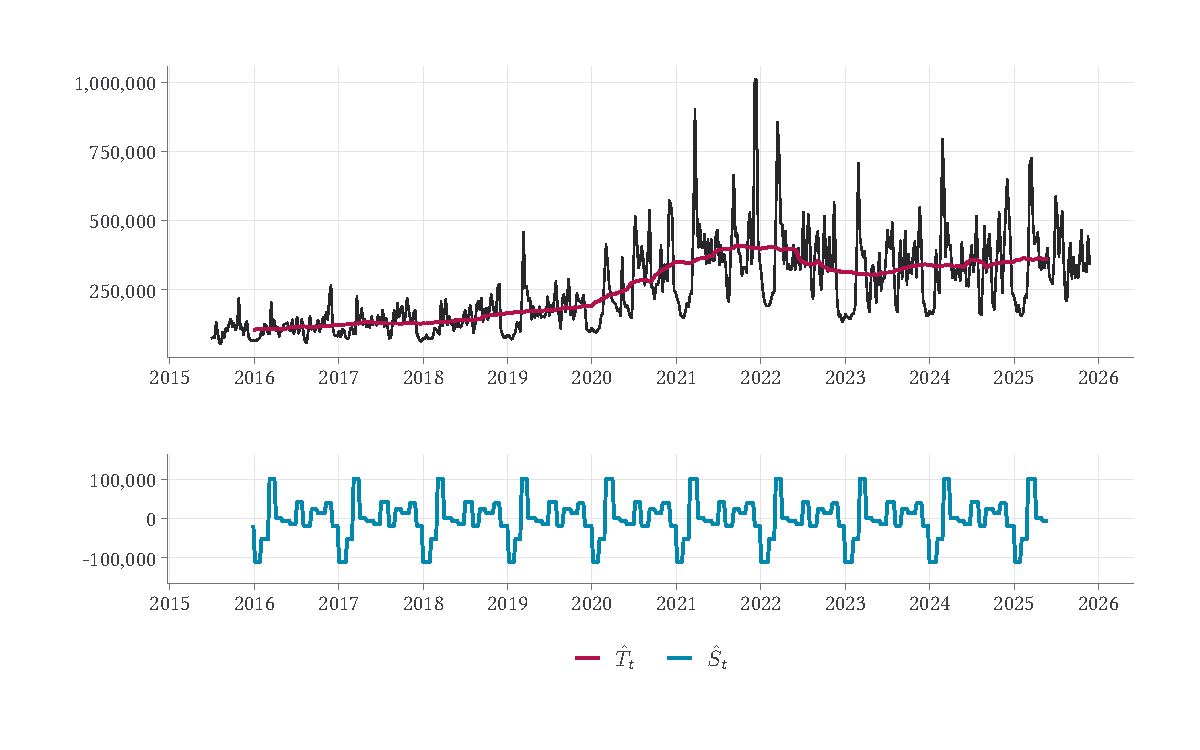
\includegraphics[width = 0.9\textwidth]{figures/p_f1_decomposition.pdf}
  \end{center}
\end{figure}

  \begin{smallcodeblock}[{}]
OLS estimation, Dep. Var.: log_views
Observations: 544
Standard-errors: Heteroskedasticity-robust
                  Estimate Std. Error t value   Pr(>|t|)
(Intercept)        -271.55      8.143   -33.3  < 2.2e-16 
year(date)            0.14      0.004    34.8  < 2.2e-16 
month::February       0.26      0.066     3.9 1.0985e-04 
month::March          0.70      0.071     9.9  < 2.2e-16 
month::April          0.42      0.059     7.1 4.6862e-12 
month::May            0.42      0.058     7.2 1.8021e-12 
month::June           0.33      0.059     5.6 3.4360e-08 
month::July           0.54      0.055     9.7  < 2.2e-16 
month::August         0.33      0.065     5.2 3.6351e-07 
month::Sepember       0.52      0.058     8.9  < 2.2e-16 
month::Octember       0.50      0.057     8.7  < 2.2e-16 
month::November       0.61      0.061     9.9  < 2.2e-16 
month::December       0.34      0.091     3.8 1.6936e-04 
is_race_week::TRUE    0.34      0.033    10.6  < 2.2e-16 
  \end{smallcodeblock}


\end{document}
